\let\negmedspace\undefined
\let\negthickspace\undefined
\documentclass[journal,12pt,onecolumn]{IEEEtran}
\usepackage{cite}
\usepackage{amsmath,amssymb,amsfonts,amsthm}
\usepackage{algorithmic}
\usepackage[version=4]{mhchem}
\usepackage{graphicx}
\usepackage{textcomp}
\usepackage{xcolor}
\usepackage{amsmath}
\usepackage{txfonts}
\usepackage{listings}
\usepackage{enumitem}
\usepackage{mathtools}
\usepackage{gensymb}
\usepackage{comment}
\usepackage[breaklinks=true]{hyperref}
\usepackage{tkz-euclide} 
\usepackage{gvv}                                        
%\def\inputGnumericTable{}                                 
\usepackage[latin1]{inputenc}     
\usepackage{xparse}
\usepackage{color}                                            
\usepackage{array}                                            
\usepackage{longtable}                                       
\usepackage{calc}                                             
\usepackage{multirow}
\usepackage{multicol}
\usepackage{hhline}                                           
\usepackage{ifthen}                                           
\usepackage{lscape}
\usepackage{tabularx}
\usepackage{array}
\usepackage{float}
\newtheorem{theorem}{Theorem}[section]
\newtheorem{problem}{Problem}
\newtheorem{proposition}{Proposition}[section]
\newtheorem{lemma}{Lemma}[section]
\newtheorem{corollary}[theorem]{Corollary}
\newtheorem{example}{Example}[section]
\newtheorem{definition}[problem]{Definition}
\newcommand{\BEQA}{\begin{eqnarray}}
\newcommand{\EEQA}{\end{eqnarray}}
\newcommand{\define}{\stackrel{\triangle}{=}}
\theoremstyle{remark}
\newtheorem{rem}{Remark}
% Marks the beginning of the document
\begin{document}
\title{gg Gate 2007}
\author{ai25btech11014-Gooty Suhas}
\maketitle
\begin{enumerate}

\item The maximum curvature of a cylindrically folded surface occurs at the
\begin{multicols}{4}
\begin{enumerate}
\item axial plane
\item fold axis
\item hinge
\item limb
\end{enumerate}
\end{multicols}
\vspace{0.5cm}

\item The plutonic equivalent of rhyolite is
\begin{multicols}{4}
\begin{enumerate}
\item diorite
\item granite
\item granodiorite
\item monzonite
\end{enumerate}
\end{multicols}
\vspace{0.5cm}

\item At a pressure of 14 kb and temperature of 600\,\textdegree C, basalt would metamorphose to
\begin{multicols}{4}
\begin{enumerate}
\item amphibolite
\item eclogite
\item greenschist
\item mafic granulite
\end{enumerate}
\end{multicols}
\vspace{0.5cm}

\item Which is the most abundant sediment in the deep sea?
\begin{multicols}{4}
\begin{enumerate}
\item Clay
\item Pebble
\item Sand
\item Silt
\end{enumerate}
\end{multicols}
\vspace{0.5cm}

\item Which of the following is an ore mineral of iron?
\begin{multicols}{4}
\begin{enumerate}
\item Manganite
\item Magnesite
\item Malachite
\item Magnetite
\end{enumerate}
\end{multicols}
\vspace{0.5cm}

\item Bajada is
\begin{multicols}{2}
\begin{enumerate}
\item an arid region landform
\item a fluvial landform
\item a glacial landform
\item an oceanic landform
\end{enumerate}
\end{multicols}
\vspace{0.5cm}

\item Which of the following does NOT lie within the Dharwar craton?
\begin{multicols}{2}
\begin{enumerate}
\item Bababudan Group
\item Closepet granite
\item Khairagarh volcanics
\item Kolar schist belt
\end{enumerate}
\end{multicols}
\vspace{0.5cm}

\item In which of the following oil and gas fields is limestone the reservoir rock?
\begin{multicols}{2}
\begin{enumerate}
\item Bombay High
\item Cambay basin
\item Cauvery basin
\item Krishna-Godavari basin
\end{enumerate}
\end{multicols}
\vspace{0.5cm}

\item In remote sensing, DTM is an abbreviation for
\begin{multicols}{2}
\begin{enumerate}
\item Day Time Mapping
\item Digital Triangulation Model
\item Digital Transverse Meridian
\item Digital Terrain Model
\end{enumerate}
\end{multicols}
\vspace{0.5cm}

\item Which is the most abundant element in the solar system?
\begin{multicols}{4}
\begin{enumerate}
\item Hydrogen
\item Iron
\item Oxygen
\item Silicon
\end{enumerate}
\end{multicols}
\vspace{0.5cm}

\end{enumerate}

\begin{enumerate}[resume]

\item Latitude correction applied for gravity data reduction is maximum at the latitude of
\begin{multicols}{4}
\begin{enumerate}
\item 0°
\item 30°
\item 45°
\item 60°
\end{enumerate}
\end{multicols}
\vspace{0.5cm}

\item The ratio of the Earth's total magnetic field at the Equator to that at the North Pole is
\begin{multicols}{4}
\begin{enumerate}
\item $\frac{4}{3}$
\item $\frac{3}{4}$
\item $\frac{2}{3}$
\item $\frac{1}{2}$
\end{enumerate}
\end{multicols}
\vspace{0.5cm}

\item The apparent resistivity type curve recorded over the following three-layer section (top - dry soil; middle - saturated aquifer; bottom - bedrock) is
\begin{multicols}{4}
\begin{enumerate}
\item A-Type
\item H-Type
\item K-Type
\item Q-Type
\end{enumerate}
\end{multicols}
\vspace{0.5cm}

\item Self-potential method is used in geophysical prospecting of ore deposits predominantly containing
\begin{multicols}{4}
\begin{enumerate}
\item chalcopyrite
\item chromite
\item ilmenite
\item magnetite
\end{enumerate}
\end{multicols}
\vspace{0.5cm}

\item Deep earthquakes are associated with
\begin{multicols}{2}
\begin{enumerate}
\item mid-oceanic ridges
\item rift zones
\item subduction zones
\item transform faults
\end{enumerate}
\end{multicols}
\vspace{0.5cm}

\item The average P-wave velocity in the continental crust is
\begin{multicols}{4}
\begin{enumerate}
\item 3.5 km/s
\item 4.5 km/s
\item 5.5 km/s
\item 6.5 km/s
\end{enumerate}
\end{multicols}
\vspace{0.5cm}

\item The amplitude of ground motion generated by an earthquake of magnitude 8 is greater than that of an earthquake of magnitude 5 by a factor of
\begin{multicols}{4}
\begin{enumerate}
\item 3
\item 100
\item 300
\item 1000
\end{enumerate}
\end{multicols}
\vspace{0.5cm}

\item A P-wave is NOT a
\begin{multicols}{2}
\begin{enumerate}
\item dilatational wave
\item irrotational wave
\item longitudinal wave
\item rotational wave
\end{enumerate}
\end{multicols}
\vspace{0.5cm}

\item Low velocity zone (LVZ) occurs globally at the base of the
\begin{multicols}{4}
\begin{enumerate}
\item asthenosphere
\item crust
\item lithosphere
\item outer core
\end{enumerate}
\end{multicols}
\vspace{0.5cm}

\item The fastest spreading divergent plate boundary is the
\begin{multicols}{2}
\begin{enumerate}
\item Carlsberg ridge
\item Central-Indian ridge
\item East Pacific rise
\item Mid-Atlantic ridge
\end{enumerate}
\end{multicols}
\vspace{0.5cm}

\item An open fold may appear to be isoclinal when viewed in a section
\begin{multicols}{2}
\begin{enumerate}
\item at a low angle to the fold axis
\item at 45° to the fold axis
\item perpendicular to the fold axis
\item parallel to the axial plane
\end{enumerate}
\end{multicols}
\vspace{0.5cm}

\item Glaucophane is a dense mineral because
\begin{enumerate}
\item Na occurs in the 'A' site while Al is in the octahedral site
\item Na occurs in the 'A' site while Al is in the tetrahedral site
\item Na occurs in the 'M4' site while Al is in the octahedral site
\item Na occurs in the 'M4' site while Al is in the tetrahedral site
\vspace{0.5cm}
\end{enumerate}


\item When a hydrous fluid infiltrates a rock containing the assemblage wollastonite + calcite + quartz at a fixed pressure and temperature, the modal proportion of
\begin{enumerate}
\item calcite will increase at the expense of quartz and wollastonite
\item wollastonite will increase at the expense of quartz and calcite
\item quartz will increase at the expense of calcite and wollastonite
\item calcite and quartz will increase at the expense of wollastonite
\vspace{0.5cm}
\end{enumerate}


\item Which of the following represents a correct magmatic fractionation sequence?
\begin{enumerate}
\item Basalt $\rightarrow$ Andesite $\rightarrow$ Dacite $\rightarrow$ Phonolite
\item Basalt $\rightarrow$ Andesite $\rightarrow$ Trachyte $\rightarrow$ Rhyolite
\item Basalt $\rightarrow$ Mugearite $\rightarrow$ Dacite $\rightarrow$ Rhyolite
\item Basalt $\rightarrow$ Mugearite $\rightarrow$ Trachyte $\rightarrow$ Phonolite
\vspace{0.5cm}
\end{enumerate}



\item In the following figure, four rocks (W, X, Y and Z) undergo fractional melting. Which rock will require the highest temperature for complete melting? (Rock Y is of eutectic composition)

\begin{figure}[h]
    \centering
    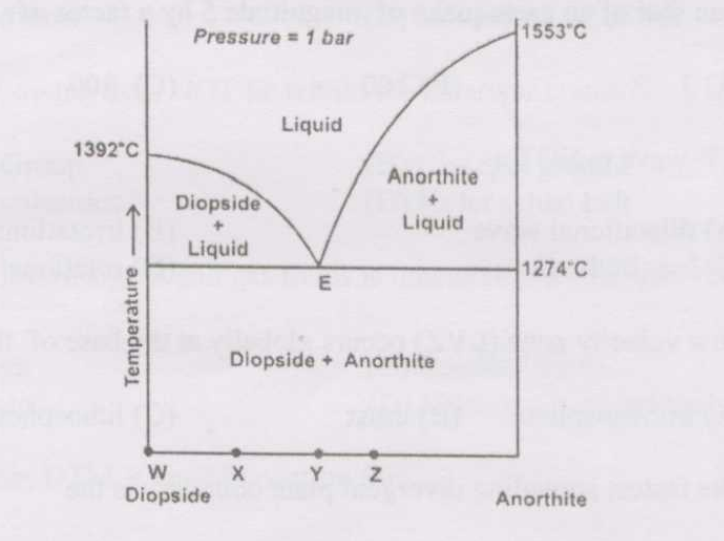
\includegraphics[width=0.8\textwidth]{figs/fig1.png}
    \caption{Image of Question 25}
    \label{fig:question25}
\end{figure}

\begin{multicols}{2}
\begin{enumerate}
\item W
\item X
\item Y
\item Z
\end{enumerate}
\end{multicols}
\vspace{0.5cm}

\item Which is the most common type of porosity in sandstone?
\begin{multicols}{4}
\begin{enumerate}
\item Mouldic
\item Intraparticle
\item Interparticle
\item Shelter
\end{enumerate}
\end{multicols}
\vspace{0.5cm}

\item Which of the following features is NOT a 'tool mark'?
\begin{multicols}{4}
\begin{enumerate}
\item Chevron mark
\item Groove cast
\item Load cast
\item Prod mark
\end{enumerate}
\end{multicols}
\vspace{0.5cm}

\item Match the following:

\noindent
\begin{minipage}[t]{0.45\textwidth}
\textbf{Group I:}  

P. Lead  

Q. Aluminium  

R. Chromite  

S. Muscovite  
\end{minipage}
\hfill
\begin{minipage}[t]{0.45\textwidth}
\textbf{Group II:}  

1. Magmatic  

2. Pegmatitic  

3. Residual  

4. Hydrothermal  
\end{minipage}

\vspace{0.3cm}

\begin{multicols}{2}
(A) P--2, Q--1, R--3, S--4  
(B) P--4, Q--3, R--1, S--2  
(C) P--3, Q--4, R--2, S--1  
(D) P--3, Q--4, R--2, S--1  
\end{multicols}
\vspace{0.5cm}

\item State the nature of the following reaction:

\ce{Si+ + 4H2O -> H4SiO4 + 4H+}

\begin{multicols}{4}
\begin{enumerate}
\item hydration
\item hydrolysis
\item oxidation
\item reduction
\end{enumerate}
\end{multicols}
\vspace{0.5cm}

\item Match the ionic species in Group I with their representative concentrations (ppm) in Group II, as found in meteoric water at 6°C.

\noindent
\begin{minipage}[t]{0.45\textwidth}
\textbf{Group I:}  

P. Na$^+$  

Q. Mg$^{2+}$  

R. Ca$^{2+}$  

S. K$^+$  
\end{minipage}
\hfill
\begin{minipage}[t]{0.45\textwidth}
\textbf{Group II:}  

1. 2.4  

2. 23.0  

3. 1.0  

4. 5.1  
\end{minipage}

\vspace{0.3cm}
\begin{enumerate}
\begin{multicols}{2}
\item P--2, Q--1, R--4, S--3  
\item P--1, Q--2, R--3, S--4  
\item P--4, Q--3, R--2, S--1  
\item P--3, Q--4, R--1, S--2  
\end{multicols}
\vspace{0.5cm}
\end{enumerate}

\item Which of the following properties does NOT affect the permeability of sandstone?
\begin{multicols}{2}
\begin{enumerate}
\item Pore size
\item Tortuosity of pores
\item Sorting
\item Mineralogy of framework grains
\end{enumerate}
\end{multicols}
\vspace{0.5cm}

\item Which of the following macerals has the lowest H/C ratio?
\begin{multicols}{4}
\begin{enumerate}
\item Alginite
\item Fusinite
\item Resinite
\item Sporinite
\end{enumerate}
\end{multicols}
\vspace{0.5cm}

\item The paleoenvironmental condition indicated by the foraminiferal assemblage, Ammonia--Cibicides--Quinqueloculina is
\begin{multicols}{4}
\begin{enumerate}
\item abyssal
\item bathyal
\item non-marine
\item shelf
\end{enumerate}
\end{multicols}
\vspace{0.5cm}
\item Match the bivalves in Group I with the dentitions in Group II.

\noindent
\begin{minipage}[t]{0.45\textwidth}
\textbf{Group I:}  

P. Nucula  

Q. Spondylus  

R. Mytilus  

S. Mya  
\end{minipage}
\hfill
\begin{minipage}[t]{0.45\textwidth}
\textbf{Group II:}  

1. Desmodont  

2. Pachydont  

3. Dysodont  

4. Taxodont  

5. Isodont  

6. Schizodont  
\end{minipage}

\vspace{0.3cm}
\begin{enumerate}
\begin{multicols}{2}
\item P--4, Q--5, R--3, S--1  
\item P--4, Q--1, R--3, S--2  
\item P--6, Q--5, R--1, S--3  
\item P--6, Q--5, R--3, S--2  
\end{multicols}
\vspace{0.5cm}
\end{enumerate}




\item Match the following stratigraphic units in Group I with their corresponding ages in Group II.

\noindent
\begin{minipage}[t]{0.45\textwidth}
\textbf{Group I:}  

P. Katrol Formation  

Q. Po Formation  

R. Kheinjua Formation  

S. Dhokpathan Formation  
\end{minipage}
\hfill
\begin{minipage}[t]{0.45\textwidth}
\textbf{Group II:}  

1. Paleozoic  

2. Archean  

3. Proterozoic  

4. Mesozoic  

5. Quaternary  

6. Tertiary  
\end{minipage}

\vspace{0.3cm}

\begin{multicols}{2}
\begin{enumerate}
\item P--6, Q--1, R--3, S--5  
\item P--4, Q--6, R--2, S--1  
\item P--1, Q--4, R--1, S--6  
\item P--4, Q--1, R--3, S--6  
\end{enumerate}
\end{multicols}
\vspace{0.5cm}

\item Match the minerals in Group I with their respective silicate structures in Group II.

\noindent
\begin{minipage}[t]{0.45\textwidth}
\textbf{Group I:}  

P. Olivine  

Q. Epidote  

R. Biotite  

S. Quartz  
\end{minipage}
\hfill
\begin{minipage}[t]{0.45\textwidth}
\textbf{Group II:}  

1. Nesosilicate  

2. Sorosilicate  

3. Inosilicate  

4. Phyllosilicate  

5. Cyclosilicate  

6. Tectosilicate  
\end{minipage}

\vspace{0.3cm}

\begin{multicols}{2}
\begin{enumerate}
\item P--1, Q--2, R--5, S--4  
\item P--1, Q--6, R--2, S--4  
\item P--3, Q--6, R--4, S--2  
\item P--4, Q--5, R--6, S--1  
\end{enumerate}
\end{multicols}
\vspace{0.5cm}

\item Match the following shear zones in Group I with their tectonic settings in Group II.

\noindent
\begin{minipage}[t]{0.45\textwidth}
\textbf{Group I:}  

P. Moyar--Bhavani Shear Zone  

Q. Kui--Chitraseni Shear Zone  

R. Nagavalli--Vamsadhara Shear Zone  

S. Jabanahalli Shear Zone  
\end{minipage}
\hfill
\begin{minipage}[t]{0.45\textwidth}
\textbf{Group II:}  

1. Eastern Ghats Mobile Belt  

2. Southern Granulite Terrain  

3. Western Dharwar Craton  

4. Aravalli--Delhi Fold Belt  

5. Singhbhum Craton  

6. Bhandara Craton  
\end{minipage}

\vspace{0.3cm}

\begin{multicols}{2}
\begin{enumerate}
\item P--1, Q--2, R--5, S--4  
\item P--6, Q--5, R--2, S--4  
\item P--4, Q--2, R--6, S--1  
\item P--2, Q--4, R--1, S--3  
\end{enumerate}
\end{multicols}
\vspace{0.5cm}

\item Which is the correct sequence of occurrence of the following thrusts in the Himalayan mountain belt along a south to north traverse?
\begin{enumerate}
\item Krol Thrust $\rightarrow$ Ramgarh Thrust $\rightarrow$ Almora Thrust $\rightarrow$ ITSZ  
\item Ramgarh Thrust $\rightarrow$ Krol Thrust $\rightarrow$ Almora Thrust $\rightarrow$ ITSZ  
\item Krol Thrust $\rightarrow$ Almora Thrust $\rightarrow$ Ramgarh Thrust $\rightarrow$ ITSZ  
\item Almora Thrust $\rightarrow$ Ramgarh Thrust $\rightarrow$ ITSZ $\rightarrow$ Krol Thrust  
\vspace{0.5cm}
\end{enumerate}

\item Which of the following triple junctions is ALWAYS stable? (R = ridge; T = trench; F = transform fault)

\begin{multicols}{4}
\begin{enumerate}
\item F--F--F  
\item R--R--R  
\item T--R--F  
\item T--T--T  
\end{enumerate}
\end{multicols}
\vspace{0.5cm}


\item Match the geomorphic features in Group I with their settings in Group II.

\noindent
\begin{minipage}[t]{0.45\textwidth}
\textbf{Group I:}  

P. Nickpoints  

Q. Pediplains  

R. Duricrust  

S. Yardangs  
\end{minipage}
\hfill
\begin{minipage}[t]{0.45\textwidth}
\textbf{Group II:}  

1. Karst topography  

2. Paleosols  

3. Moraine  

4. Rejuvenation  

5. Desert  

6. Abrasion  
\end{minipage}

\vspace{0.3cm}

\begin{multicols}{2}
\begin{enumerate}
\item P--1, Q--2, R--5, S--4  
\item P--4, Q--5, R--2, S--6  
\item P--6, Q--5, R--2, S--3  
\item P--5, Q--3, R--1, S--2  
\end{enumerate}
\end{multicols}
\vspace{0.5cm}

\item A straight, steep mountain front, with little penetration of the alluvial fans into the range suggests the following:

\begin{multicols}{2}
\begin{enumerate}
\item wind erosion  
\item slow uplift along an active fault  
\item rapid uplift along an active fault  
\item the presence of ancient inactive fault  
\end{enumerate}
\end{multicols}
\vspace{0.5cm}

\item At a fixed temperature, find the concentration (mole/litre) of ferric ion in solution if  
(i) solubility product of ferric hydroxide $K = 10^{-38.6}$  
(ii) ionisation product of water $K_w = 10^{-14.2}$  
(iii) pH = 7

\begin{multicols}{4}
\begin{enumerate}
\item $10^{-17}$  
\item $10^{-7}$  
\item $10^{+7}$  
\item $10^{+17}$  
\end{enumerate}
\end{multicols}
\vspace{0.5cm}

\item A basaltic lava flow is found to have a $^{87}\text{Sr}/^{86}\text{Sr}$ ratio of 0.720, and a $^{87}\text{Rb}/^{86}\text{Sr}$ ratio of 0.750. If the initial $^{87}\text{Sr}/^{86}\text{Sr}$ value is determined to be 0.704, what is the age of the flow? (Assume $\lambda = 1.42 \times 10^{-11}$ year$^{-1}$)

\begin{multicols}{4}
\begin{enumerate}
\item $2.5 \times 10^9$ years  
\item $1.5 \times 10^9$ years  
\item $2.5 \times 10^1$ years  
\item $1.5 \times 10^1$ years  
\end{enumerate}
\end{multicols}
\vspace{0.5cm}

\item What are the normal ($\sigma_n$) and shear ($\tau$) stresses acting on a plane that makes an angle of 30° with the maximum principal compressive stress ($\sigma_1$) direction? Given $\sigma_1 = 10$ kb and $\sigma_2 = 5$ kb.

\begin{multicols}{2}
\begin{enumerate}
\item $\sigma_n = 5.25$ kb; $\tau = 1.17$ kb  
\item $\sigma_n = 6.25$ kb; $\tau = 2.17$ kb  
\item $\sigma_n = 7.25$ kb; $\tau = 3.17$ kb  
\item $\sigma_n = 8.25$ kb; $\tau = 4.17$ kb  
\end{enumerate}
\end{multicols}
\vspace{0.5cm}

\item Quartz can be optically distinguished from nepheline based on

\begin{multicols}{2}
\begin{enumerate}
\item relief  
\item birefringence  
\item optic sign  
\item extinction angle  
\end{enumerate}
\end{multicols}
\vspace{0.5cm}

\item The Poisson's ratio of a rock with P-- and S--wave velocities in the ratio of 3:1 is

\begin{multicols}{4}
\begin{enumerate}
\item 0.20  
\item 0.25  
\item 0.30  
\item 0.35  
\end{enumerate}
\end{multicols}
\vspace{0.5cm}

\item A seismic reflection segment after migration
\begin{enumerate}

\item shallows and steepens  
\item deepens and steepens  
\item lengthens and deepens  
\item shortens and deepens  
\vspace{0.5cm}
\end{enumerate}

\item The coverage obtained for a 12--geophone CDP profile with shot spacing equal to twice the geophone spacing is

\begin{multicols}{4}
\begin{enumerate}
\item 3--fold  
\item 6--fold  
\item 12--fold  
\item 24--fold  
\end{enumerate}
\end{multicols}
\vspace{0.5cm}

\item A P--wave incident on a horizontal interface between two layers at an angle of 30° generates a reflected S--wave. What is the angle of reflection of the S--wave? (The P-- and S--wave velocities in the top layer are 4 km/s and 2.5 km/s respectively).

\begin{multicols}{4}
\begin{enumerate}
\item 12°  
\item 14°  
\item 16°  
\item 18°  
\end{enumerate}
\end{multicols}
\vspace{0.5cm}

\item The decimal number 27 is represented in binary form as

\begin{multicols}{4}
\begin{enumerate}
\item 11101  
\item 11001  
\item 10111  
\item 11011  
\end{enumerate}
\end{multicols}
\vspace{0.5cm}

\item A salt dome is characterized by
\begin{enumerate}

\item low velocity and low density  
\item low velocity and high density  
\item high velocity and low density  
\item high velocity and high density  
\vspace{0.5cm}
\end{enumerate}

\item Convolving two sampled signals $f(n) = \{1,1,2,2\}$ with $g(n) = \{3,2,1\}$ results in a function $x(n)$ equal to

\begin{multicols}{2}
\begin{enumerate}
\item \{1, 3, 7, 9, 10, 6\}  
\item \{3, 5, 9, 11, 6, 2\}  
\item \{3, 9, 6, 11, 2, 2\}  
\item \{3, 5, 9, 6, 11, 5\}  
\end{enumerate}
\end{multicols}
\vspace{0.5cm}

\item Arrange the following EM methods in order of increasing depth of investigation:  
P -- Very Low Frequency method  
Q -- Magnetotelluric method  
R -- Ground Penetrating Radar method  
S -- Slingram method

\begin{multicols}{4}
\begin{enumerate}
\item P < R < S < Q  
\item S < R < P < Q  
\item R < P < S < Q  
\item P < R < Q < S  
\end{enumerate}
\end{multicols}
\vspace{0.5cm}

\item Which of the following is measured in the time domain Induced Polarization method?
\begin{enumerate}

\item Transient decay of electric potential  
\item Electric current injected into the ground  
\item Electric potential and injected current  
\item DC resistance only  
\vspace{0.5cm}
\end{enumerate}

\item In magnetotelluric method, EM source field is

\begin{multicols}{2}
\begin{enumerate}
\item a plane wave source  
\item a spherical wave source  
\item a cylindrical wave source  
\item an elliptical wave source  
\end{enumerate}
\end{multicols}
\vspace{0.5cm}

\item In magnetotelluric method, phase angle derived from measured data over a homogeneous medium is

\begin{multicols}{4}
\begin{enumerate}
\item 0°  
\item 30°  
\item 45°  
\item 90°  
\end{enumerate}
\end{multicols}
\vspace{0.5cm}

\item For a fixed electrode spacing, arrange the following electrode configurations in the order of increasing depth of investigation:  
P -- Schlumberger  
Q -- Wenner  
R -- Three electrodes  
S -- Two electrodes

\begin{multicols}{4}
\begin{enumerate}
\item P < Q < S < R  
\item P < R < S < Q  
\item P < R < Q < S  
\item P < Q < R < S  
\end{enumerate}
\end{multicols}
\vspace{0.5cm}

\item The correct expression relating the gravitational ($U$) and magnetic ($W$) potentials is  
(G = universal gravitational constant, $\rho$ = density, $I$ = intensity of magnetization, $\alpha$ = direction of magnetization)

\begin{multicols}{2}
\begin{enumerate}
\item $W = -\dfrac{I}{G\rho} \dfrac{\partial U}{\partial \alpha}$  
\item $W = -\dfrac{\rho}{G} \dfrac{\partial U}{\partial I}$  
\item $U = -\dfrac{\rho}{G} \dfrac{\partial W}{\partial I}$  
\item $U = -\dfrac{I}{G\rho} \dfrac{\partial W}{\partial \alpha}$  
\end{enumerate}
\end{multicols}
\vspace{0.5cm}

\item Magnetic survey was conducted from 8:00 A.M. to 12:00 noon. Observations:

\begin{center}
\begin{tabular}{|c|c|c|c|c|c|c|}
\hline
Station No & 1 (Base) & 2 & 3 & 4 & 5 & 1 (Base) \\
\hline
Time & 8:00 & 9:00 & 10:00 & 11:00 & 12:00 & 12:00 \\
\hline
Total field ($\gamma$) & 45500 & 45650 & 45750 & 45850 & 45850 & 45700 \\
\hline
\end{tabular}
\end{center}

Which station shows the maximum anomaly after linear drift correction?

\begin{multicols}{4}
\begin{enumerate}
\item 2  
\item 3  
\item 4  
\item 5  
\end{enumerate}
\end{multicols}
\vspace{0.5cm}

\item At 45N latitude, a spherical body having a radius 500 m, density 3.5 g/cc and magnetic susceptibility $5.0 \times 10^{-6}$ CGS unit, lies at a depth of 1.0 km. Assuming present--day magnetic field, which statement is true if measurements are made along an E--W profile?
\begin{enumerate}

\item Both gravity and total magnetic field anomalies are symmetric  
\item Gravity anomaly is symmetric and total magnetic field anomaly is asymmetric  
\item Total magnetic field anomaly is symmetric and gravity anomaly is asymmetric  
\item Both gravity and total magnetic field anomalies are asymmetric  
\vspace{0.5cm}
\end{enumerate}

\item Match the following:

\noindent
\begin{minipage}[t]{0.45\textwidth}
\textbf{Group I:}  

P. Paramagnetic  

Q. Diamagnetic  

R. Ferromagnetic  

S. Antiferromagnetic  
\end{minipage}
\hfill
\begin{minipage}[t]{0.45\textwidth}
\textbf{Group II:}  

1. Cobalt  

2. Ilmenite  

3. Pyroxene  

4. Quartz  
\end{minipage}

\vspace{0.3cm}

\begin{multicols}{2}
\begin{enumerate}
\item P -- 2, Q -- 3, R -- 1, S -- 4  
\item P -- 1, Q -- 3, R -- 2, S -- 4  
\item P -- 4, Q -- 2, R -- 1, S -- 3  
\item P -- 3, Q -- 4, R -- 1, S -- 2  
\end{enumerate}
\end{multicols}
\vspace{0.5cm}






\item The difference in gravity measurements aboard two ships sailing towards each other in opposite directions (E--W) with a constant speed of 10 knots is 130 mgal at the crossing point of both the ships. At what latitude are the ships sailing?

\begin{multicols}{4}
\begin{enumerate}
\item 15°  
\item 30°  
\item 45°  
\item 60°  
\end{enumerate}
\end{multicols}
\vspace{0.5cm}

\item After decaying through 7 half--life periods, the original amount of radioactive substance that reduces to an amount of 64 is

\begin{multicols}{4}
\begin{enumerate}
\item 0.25 g  
\item 0.50 g  
\item 1.0 g  
\item 2.0 g  
\end{enumerate}
\end{multicols}
\vspace{0.5cm}

\item Number of atoms and disintegration constants of the parent ($N_1$, $\lambda_1$) and daughter ($N_2$, $\lambda_2$) radionuclides respectively in secular equilibrium are related as

\begin{multicols}{2}
\begin{enumerate}
\item $N_1 = \lambda_2 N_2$  
\item $N_1 \lambda_1 = N_2 \lambda_2$  
\item $N_1 = N_2 \lambda_2$  
\item $N_1 \lambda_1 = \lambda_2 N_2$  
\end{enumerate}
\end{multicols}
\vspace{0.5cm}

\item What is the volume (\%) of shale in a shaly--sand bed exhibiting a pseudo--static SP of --44 mV? (Static SP for clean sand = --55 mV)

\begin{multicols}{4}
\begin{enumerate}
\item 10  
\item 20  
\item 30  
\item 40  
\end{enumerate}
\end{multicols}
\vspace{0.5cm}

\item If the saturation exponent in Archies equation is 2, the bulk resistivity of 50\% water saturated formation increases in comparison to that of a fully water saturated formation by a factor of

\begin{multicols}{4}
\begin{enumerate}
\item 4  
\item 8  
\item 16  
\item 32  
\end{enumerate}
\end{multicols}
\vspace{0.5cm}

\item Determination of formation porosity using neutron logging is based on

\begin{multicols}{2}
\begin{enumerate}
\item chlorine index  
\item hydrogen index  
\item neutron activation index  
\item oxygen index  
\end{enumerate}
\end{multicols}
\vspace{0.5cm}

\item Which combination of logs is used to identify a gas zone based on the characteristic shape of the derived porosity plots?

\begin{multicols}{2}
\begin{enumerate}
\item Sonic and density  
\item Resistivity and density  
\item Density and neutron  
\item Sonic and neutron  
\end{enumerate}
\end{multicols}
\vspace{0.5cm}

\item Inverse solution for an underdetermined problem can be constructed by

\begin{multicols}{2}
\begin{enumerate}
\item minimum norm inversion  
\item least square inversion  
\item regularized least square inversion  
\item Marquardt inversion  
\end{enumerate}
\end{multicols}
\vspace{0.5cm}

\item Primary field source used in Slingram EM method is a

\begin{multicols}{2}
\begin{enumerate}
\item small circular loop  
\item large rectangular loop  
\item long grounded wire  
\item long vertical transmitter  
\end{enumerate}
\end{multicols}
\vspace{0.5cm}

\subsection*{Common Data for Questions 71,72,73:}
A P--wave generated from a surface source is incident at an angle of 15° on the horizontal interface between two 100 m thick layers with velocities $V_1 = 2$ km/s and $V_2 = 4$ km/s for the first and second layers respectively.
\vspace{0.5cm}

\item The crossover distance (metres) for a head wave from the interface between two layers is  
Given: P--wave incident at 15°, layer thickness = 100 m, $V_1 = 2$ km/s, $V_2 = 4$ km/s

\begin{multicols}{4}
\begin{enumerate}
\item 326  
\item 336  
\item 346  
\item 356  
\end{enumerate}
\end{multicols}
\vspace{0.5cm}

\item A reflection from the base of the second layer is recorded at an offset (source--receiver) distance (metres) of

\begin{multicols}{4}
\begin{enumerate}
\item 160  
\item 165  
\item 170  
\item 175  
\end{enumerate}
\end{multicols}
\vspace{0.5cm}

\item The total travel time (ms) taken for the P--wave generated at the surface to reach the detector after reflection from the base of the second layer is

\begin{multicols}{4}
\begin{enumerate}
\item 152  
\item 157  
\item 162  
\item 167  
\end{enumerate}
\end{multicols}
\vspace{0.5cm}

\end{enumerate}





\subsection*{Common Data for Questions 74, 75:}
The figure below represents the geological map of an area. Based on the map, attempt questions 74 and 75. Contours depicted are in metres.


\begin{figure}[H]
    \centering
    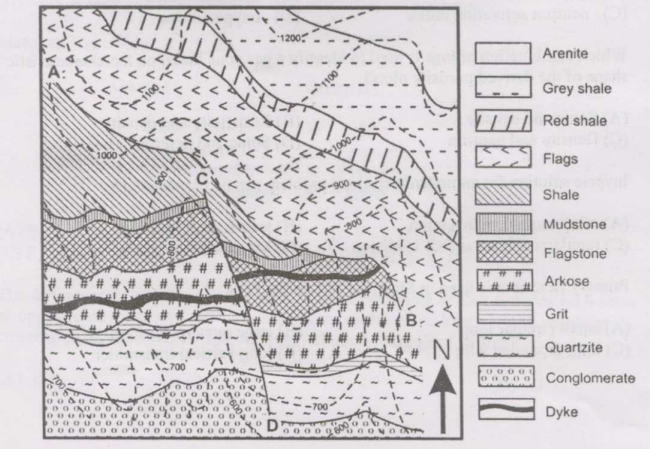
\includegraphics[width=0.8\textwidth]{figs/fig2.png}
    \caption{Image for questions 74,75}
    \label{fig:question25}
\end{figure}

\begin{enumerate}[resume]
\item What is the nature of the discontinuity AB (based on geological map)?
\begin{enumerate}

\item Fault  
\item Disconformity  
\item Paraconformity  
\item Angular unconformity  
\vspace{0.5cm}
\end{enumerate}

\item The discontinuity CD represents a
\begin{enumerate}

\item normal fault  
\item reverse fault  
\item strike-slip fault  
\item strike fault  
\vspace{0.5cm}
\end{enumerate}

\subsection*{Statement for Linked Answer Questions 76 and 77:}
\end{enumerate}
\vspace{0.5cm}

The discontinuities within the earth are marked by changes in velocity and density of the medium.
\vspace{0.5cm}

\begin{enumerate}[resume]

\item The velocity discontinuity within the earth at which the density of the medium is closest to the average density of the earth is

\begin{multicols}{4}
\begin{enumerate}
\item Conrad  
\item Gutenberg  
\item Lehmann  
\item Mohorovicic  
\end{enumerate}
\end{multicols}
\vspace{0.5cm}

\item The change in P-wave velocity across the above discontinuity is

\begin{multicols}{4}
\begin{enumerate}
\item 1.7 km/s  
\item 3.7 km/s  
\item 5.7 km/s  
\item 7.7 km/s  
\end{enumerate}
\end{multicols}
\vspace{0.5cm}

\subsection*{Statement for Linked Answer Questions 78 and 79:}
\end{enumerate}
\vspace{0.5cm}

In electromagnetic method of geophysical prospecting, the depth of investigation (skin depth), is a function of the physical property of the medium and frequency of the source field.
\vspace{0.5cm}

\begin{enumerate}[resume]

\item The expression for skin depth $\delta$ in a homogeneous medium with conductivity $\sigma$, magnetic permeability $\mu$, and angular frequency $\omega$ is

\begin{multicols}{4}
\begin{enumerate}
\item $\delta = \sqrt{\dfrac{2}{\omega \mu \sigma}}$  
\item $\delta = \dfrac{1}{\omega \mu \sigma}$  
\item $\delta = \dfrac{1}{\sqrt{\omega \mu \sigma}}$  
\item $\delta = \sqrt{\omega \mu \sigma}$  
\end{enumerate}
\end{multicols}
\vspace{0.5cm}

\item The frequency of the EM source required to achieve a depth of investigation of 1 km in a medium of electrical resistivity of 4.0 $\Omega$m and magnetic permeability of $4\pi \times 10^{-7}$ H/m is

\begin{multicols}{4}
\begin{enumerate}
\item 1 Hz  
\item 10 Hz  
\item 100 Hz  
\item 1000 Hz  
\end{enumerate}
\end{multicols}
\vspace{0.5cm}

\subsection*{Statement for Linked Answer Questions 80 \& 81:}
\end{enumerate}
\vspace{0.5cm}

Paleocurrent data for a sedimentary succession is as follows:
\vspace{0.5cm}
$$N\,20^\circ\,E,\ N\,25^\circ\,E,\ N\,30^\circ\,E,\ N\,15^\circ\,E,\ S\,20^\circ\,W,\ S\,25^\circ\,W,\ S\,30^\circ\,W,\ S\,15^\circ\,W,\ N\,25^\circ\,E,\ S\,25^\circ\,W$$

\begin{enumerate}[resume]

\item The rose diagram generated from the paleocurrent data is

\begin{multicols}{2}
\begin{enumerate}
\item bimodal -- bipolar  
\item polymodal  
\item trimodal  
\item unimodal  
\end{enumerate}
\end{multicols}
\vspace{0.5cm}

\item Which environment of deposition can explain the above paleocurrent data?

\begin{multicols}{4}
\begin{enumerate}
\item Alluvial fan  
\item Deep marine  
\item Fluvial  
\item Tidal flat  
\end{enumerate}
\end{multicols}
\vspace{0.5cm}

\subsection*{Statement for Linked Answer Questions 82 \& 83:}
\end{enumerate}
\vspace{0.5cm}

A garnet peridotite contains 60\% olivine, 25\% orthopyroxene, 10\% clinopyroxene, and 5\% garnet. The partition coefficients ($K_p$) for cerium during melting are: olivine = 0.001, orthopyroxene = 0.003, clinopyroxene = 0.1, and garnet = 0.02.
\vspace{0.5cm}

\begin{enumerate}[resume]

\item During melting of the garnet peridotite, the bulk distribution coefficient of cerium is  
Given:  
Olivine -- 60\% -- $K_D = 0.001$  
Orthopyroxene -- 25\% -- $K_D = 0.003$  
Clinopyroxene -- 10\% -- $K_D = 0.1$  
Garnet -- 5\% -- $K_D = 0.02$

\begin{multicols}{4}
\begin{enumerate}
\item 0.0124  
\item 0.1240  
\item 8.0650  
\item 83.3300  
\end{enumerate}
\end{multicols}
\vspace{0.5cm}

\item The extent of equilibrium partial melting required to double the concentration of cerium in the melt compared to the source is

\begin{multicols}{4}
\begin{enumerate}
\item 5\%  
\item 20\%  
\item 35\%  
\item 50\%  
\end{enumerate}
\end{multicols}
\vspace{0.5cm}

\subsection*{Statement for Linked Answer Questions 84 \& 85:}
\end{enumerate}
\vspace{0.5cm}
A dipping limestone bed with a true width of 5 metres shows an apparent width of 10 metres on a horizontal surface.
\begin{enumerate}[resume]


\item  What is the true dip of the limestone bed?

\begin{multicols}{4}
\begin{enumerate}
\item 70°  
\item 50°  
\item 30°  
\item 10°  
\end{enumerate}
\end{multicols}
\vspace{0.5cm}

\item At what horizontal distance (metres) from the exposed upper surface of the bed should a vertical drill hole be made so as to intersect the top of the bed at a depth of 100 metres?

\begin{multicols}{4}
\begin{enumerate}
\item 73.2  
\item 173.2  
\item 273.2  
\item 373.2  
\end{enumerate}
\end{multicols}
\vspace{0.5cm}

\end{enumerate}

\end{document}
